\documentclass[9pt,twoside,lineno]{pnas-new}
% Use the lineno option to display guide line numbers if required.

\templatetype{pnassupportinginfo}
%\readytosubmit %% Uncomment this line before submitting, so that the instruction page is removed.

\title{The Wisdom of Threads}
\author{Robin Engelhardt, Vincent F. Hendricks}
\correspondingauthor{Robin Engelhardt.\\E-mail: robin.engelhardt@gmail.com}

\begin{document}

%% Comment/remove this line before generating final copy for submission
%\instructionspage  

\maketitle

%% Adds the main heading for the SI text. Comment out this line if you do not have any supporting information text.
\SItext

\subsection*{Data Collection}
Online labor markets and crowdsourcing platforms like Amazon Mechanical Turk (AMT) have become highly valued tools for social scientists who wish to conduct experimental research on the real time dynamics of large groups. AMT has repeatedly been shown to meet or exceed the standards set by data collection methods using other means \cite{berinsky2012evaluating, buhrmester2018evaluation}. The platform provides an integrated participant compensation system, has a large participant pool, and has been shown to be reliable, replicable, and significantly more diverse than typical American college samples \cite{mason2009financial, buhrmester2011amazon, crump2013evaluating, rand2012promise, horton2011online}.

\subsection*{Experimental Setup}
Our experimental setup on AMT is simple. After accepting our ‘HIT’ (‘human intelligence task’) and providing informed consent, participants are asked to wait in a ‘waiting room’ until the ‘choice room’ (through which all participants have to go sequentially) becomes available. After entering the choice room for the ox-experiment, participants are asked to take a look at the image and make an estimate (see screenshots in figures S1 and S2).

Depending on the view condition, participants can see $v$ preceding estimates. We chose to present the ‘oldest’ previous estimate on the top of the list and the last estimate made on the bottom. When dealing with news, or financial data, users typically want to see the most recent activity first (think tweets, online banking transactions, news updates). With conversations it is different because there is a context to consider of whatever message came before and after the one you are looking at (think blogs or facebook comments). We have chosen to use the conversation thread design (oldest on top) because there is no particular news criteria when guessing the weight of an ox or estimating the number of dots on a screen.

Participants have one minute to think about the image and make their estimate. This might sound as a severe time constraint, but exploratory trials have shown that participants in general use less than a minute when performing this task. Since participants come from all over the world, they can submit their estimate in units of kilo or in units of pounds. After submission, participants are thanked for their participation and the experiment ends. Waiting times are compensated with \$0.20 per minute (maximally 5 minutes), participation fee is \$0.10, and a bonus of \$1 is paid if an estimate is within 10\% of the true weight of the ox.

\subsection*{AMT Settings}
When working with AMT it is important to consider the right settings in order to get the best data quality possible \cite{chandler2016conducting}. Fair wage, attrition rates, removal of duplicate participants and informative feedback are some of the most important issues to address.

Average wage for participants in our experiments was $\sim$ \$12 per hour, which is considered good according to AMT guidelines and certainly above the estimated average of \$6 per hour when excluding un-submitted and rejected work \cite{hara2018data}.

Quitting a study before completing it is prevalent on AMT, and varies systemically across experimental conditions \cite{zhou2016pitfall}. For the ox-experiments attrition rates were between 20-40\% due to an unanticipated large amount of participants accepting the HIT in the first few minutes. On average 20 participants accepted our HITs within the first minute; after 10 minutes the average acceptance rate had dropped to 2-3 participants per minute and after an hour to less than one participant per minute. Our scripts were coded in such a way that participants were automatically assigned to a ‘waiting room’ in which they were asked to wait for maximally five minutes before entering the choice room. This meant that a lot of participants waited in vain. Due to such a high attrition rate in the first couple of experiments we changed the script slightly later on: Now the waiting room could contain a maximum of five participants, and when the waiting room was full, participants were told to come back and finish the HIT at a later point in time. This reduced the attrition rate to 10.5\% on average.

All participants automatically received an image-specific qualification when accepting a HIT. This qualification ensured that participants could not accept any other HITs that use the same image. Further data inspection showed that 33 participants somehow managed to accept two HITs with the same image anyway. The reason may be that the time interval between accepting two HITs with the same image was too short for the qualification to register in the AMT interface. All 33 duplicate participants were removed before data analysis. In addition, we set the qualification that participants should have completed at least 100 HITs and have an accepted HIT rate of 98\% or above. This ensured that we would get only experienced and qualified participants.

AMT participant attention was expected to be equal to or better than undergraduate participant’s attention (6), while various forms of dishonesty (practical joking or telling others about the true value offline or on an AMT participants web page) was expected to be rare. Our screening of data files before data analyses revealed that a small fraction of participants consequently submitted ridiculously high estimates across images seen, thereby skewing thread averages substantially. These estimates were not treated differently, however, because we had no reason to conclude that they were made with bad intent.

During our experiments, participants had easy access to our email for questions and possible bug reports. Apart from some minor difficulties when typing from a mobile device (less than 1\%) participants had few comments or complaints.

\subsection*{Code and Software}
All experiments are coded in the experimental software otree 2.1 \cite{chen2016otree} which is based on python and django. The code itself is designed along the same lines as the classical information cascade experiments by Anderson and Holt \cite{anderson1997information}. The main feature of any cascade game is that decisions are taken sequentially. A player makes an estimate, and the next one receives the information about the estimate of the previous player (or all or some previous players). Thus, the main technical issue is that only one person at a time can make a decision while others wait. As soon as a player finishes and leaves the choice page, the next player enters while all subsequent players still have to wait. Scripts for the analysis of data and for the plotting of all figures in the main text as well as in the Supplementary Information are available on \href{https://github.com/gavstrik/WoT}{github}.

\subsection*{Data Distributions and Trimming}
In the ox-experiments we obtained a total of 2534 estimates from 2534 unique participants. In the dots-experiments we obtained a total of 8274 estimates from 4285 unique participants. Any dot-image was only seen once by a participant, i.e. we had a total of 2141 participants seeing only one image, 842 participants seeing two images, 759 participants seeing three images, and 543 participants seeing all four images. See table \ref{table:S1} for a full list of threads and their summary statistics. 

Previous work has shown that distributions of independent estimates are approximately log-normal. Consequently, the arithmetic mean is usually much larger than most estimates and often larger than the true value. Testing our data we find distributions to be only approximately log-normal (see QQ-plots in figure S3 for examples). In addition, table \ref{table:S1} shows highly variable distributions of estimates. Skewnesses and kurtoses, describing the lack of symmetry and the size of the tail of the distributions, span values from close to zero to above 100. These asymmetries are reflected by the presence of outliers. 

For all reported aggregate measures, outliers are removed if they have an error rate above 10, so that $|x_r-truth|/truth <10$, where $x_r$ is the estimate by participant $r$. We also use a lower bound of $truth/10$, due some reports of not being able to see the form input on mobile devices or unanticipated timeouts (see SI Appendix, section “AMT Settings”). With these trimming criteria in place, we count a the following number of outliers: In the dots-experiments, 62 participants have an error rate above 100, and 118 participants have an error rate above 10, while 33 participants have made an estimate below 10\% of the true value. In the ox-experiments, one participant has an error rate above 30 and 9 participants have an error rate above 10, while 94 participants have made an estimate less than 10\% of the true value. This give a total of 151 (1.8 \%) outliers in the dots-experiments and 103 (4.1 \%) outliers in the ox-experiments, giving a grand total of 254 (2.4 \%) outliers out of 10.808 estimates.

\subsection*{Wiser Threads}
A Wisdom of Crowds-effect seems to be at work for every estimate being done: Individuals look at the distribution of previous estimates (their sample) and choose to be closer to one estimate rather than another, and mostly this chosen estimate is close to the mean or the median of the sample (see figure S5). Thus, participants aggregate social information and use it as a yardstick for their own decision. How this aggregation is performed more precisely is a matter of debate \cite{rader2017advice}, but no matter which aggregation strategy participants employ, any averaging by itself reduces the diversity of the resulting sampling distribution because the central limit theorem secures that any sampling distribution obtained from sample means will approach a normal distribution for larger sample size, irrespective of the shape of the underlying distribution.

To better understand how threads may get wiser, figure S4 shows the fraction of estimates with a higher/same/lower relative error compared to the mean relative error of the sample. Individual error is smaller than the mean error of their sample $\sim$ 60\% of the time when averaging across all $v$. This means that participants most of the time are able to use the information contained in their sample for their own calibration process and become better than chance at making an improved estimate. Now, how much better are subsequent estimates? The data shows that the mean improvement of subsequent estimates is between 0 and 1\%, as indicated by the yellow line with markers in figure S4.  Such small improvements might not sound like much but may translate into a substantial change for long threads due to their cumulative effects.

\subsection*{Variance of sample estimates}
On average, 2/3rds of all estimates in experiments with $v \in \{3,9\}$ are within the range spanned by the preceding estimates seen - i.e. higher than the lowest and lower than the highest estimate seen (54\% for $v=3$ and 81\% for $v=9$). Plotting a histogram of participant's error rates relative to the error of sample means and medians shows that a large majority of estimates are close or very close to the average or median of their sample, see figure S5. The slightly higher bars for the sample median (red) on the lower end of the x-axis may indicate that participants are more prone to anchor their own estimate on the mid-most estimate seen, rather than mentally trying to calculate an average of all the preceding estimates seen.

\subsection*{Minimum Spanning Trees}
Figure S6 depicts two spanning trees with a dots-thread on the left and an ox-thread on the right, both with $v=3$. The branches of the ox-thread on the right are more sparse and vertically aligned than the branches on the left. This indicates that herding is much more pronounced when participants estimate the weight of an ox. Figure S7 shows this effect even more clearly: while the dots-thread on the left is bushy and thick, the ox-thread on the right is fastigate and thinly scattered. 

\subsection*{Simulation Analysis}
Fig. S8 shows results of the simulation analysis as described under the Materials and Methods section in the main text. The idea is to test whether the greater accuracy of high-influencers may be due some kind of naïve social learning of participants averaging the estimates they can see, rather than to an non-naïve ability to endorse estimates that are more accurate. To do so, we first simulate how the aggregate measures of a thread perform when all participants take a weighted average of preceding estimates and their own initial (independent) \'hunch\' (looking at the histogram of the relative error rates between individual estimates and their sample means/medians, fig. S5, shows that this may not be an unreasonable approximation). This can be expressed by $$x_r = \frac{1}{v+1} \Big(e_r + \sum_{i=1}^{v} x_{r-i}\Big),$$ where $x_r$ is an actual estimate in a thread with $r \in N$, $e_r$ is a participants\' tentative guess (\'hunch\') without social information, $x_{r-i}$ are the estimates seen, and $v$ is the view count. Such a model can be taken as a special case of deGroot learning in which the network is a directed acyclic graph with $v$ edges for each node. Simulations of the model, using estimates from the control thread ($v=0$) as \'hunches\' show that the median of the sampling distribution will approach the population mean of the control thread for increasing $v$, see figure S8, which tells us that at least a partial reason for the wiser threads seen in the experiments is due to central limit effects of participants choosing an intermediate estimate among the estimates seen in their sample. 

Next, we calculate the social influence scores from the simulated data, and the result is shown in fig. S9. It reveals that the mean relative errors of the high- and low-influencers are more or less indistinguishable, telling us that a simple naive social learning process of averaging preceding estimates will not by itself create a hierarchy of influencers in a thread. There must be an additional process at work - a process that can discriminate between better and worse estimates.  

\subsection*{Compounding effects of high-influencers}
Since higher individual estimation accuracy translates into higher social influence among succeeding participants in a thread, there should be a discernible average improvement in the accuracy of participants who enter a thread at a later stage. And indeed, inspecting visually the minimum spanning trees of treatments with high $d$ and high $v$ reveals that threads tend to start with low estimates, but after 20-50 additional entries, estimates become more randomly distributed around the final aggregate values (see for instance the running medians and means in Fig. 3 in the main text and in Figs. S6-S7). 

We quantify the differences between the effects of 1) seeing $v$ independent estimates, and 2) seeing $v$ preceding estimates (which are dependent due to the compounding effect of high-influencers) by running an additional experiment (method = \'file\', session \'699h8rze\' in table S1) in which participants see nine random estimates drawn with replacement from the control condition ($v=0$). The resulting summary statistics of such a manipulated thread is shown in the middle of Fig. S10 together with the control condition ($v=0$, bottom) and the normal, unmanipulated condition ($v=9$, \'history\', top). As can be seen, there is a significant improvement in the collective performance compared to the control ($p<0.001$, Wilcoxon-Mann-Whitney test), but also a significantly worse collective performance compared to the unmanipulated \'history\'-treatment ($p<0.001$, Wilcoxon-Mann-Whitney test). This shows that seeing other peoples\' independent estimates does improve individual as well as collective performance, but seeing preceding peoples \textit{dependent} estimates in a thread improves individual as well as collective performance even more.

%%% Each figure should be on its own page
\begin{figure}
\centering
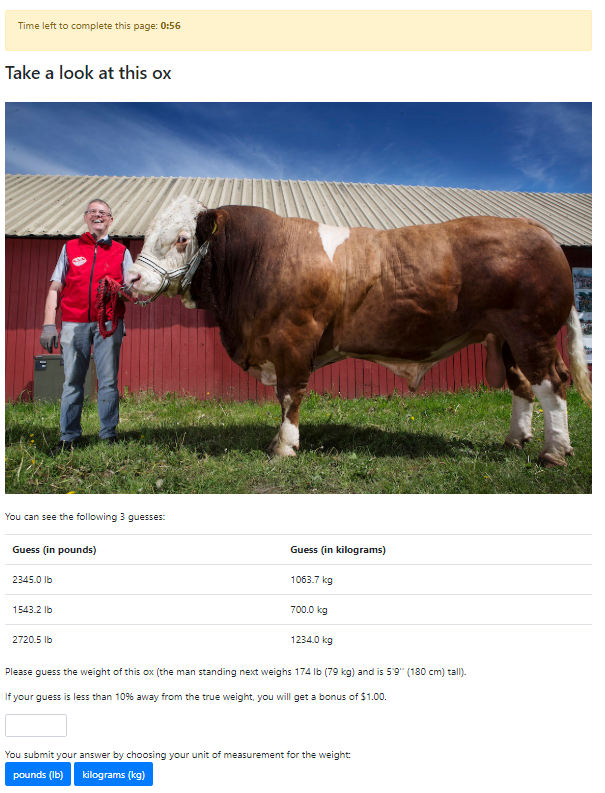
\includegraphics[width=.8\textwidth]{C:/Users/hjl161/Documents/Papers/WoT_github/images/FigS1.png}
\caption{Screendump of the choice-page in the ox-experiments with $v=3$. On image: The ox Hansi and his owner Mogens. Photo Credits: Klaus Holsting.}
\end{figure}

\begin{figure}
\centering
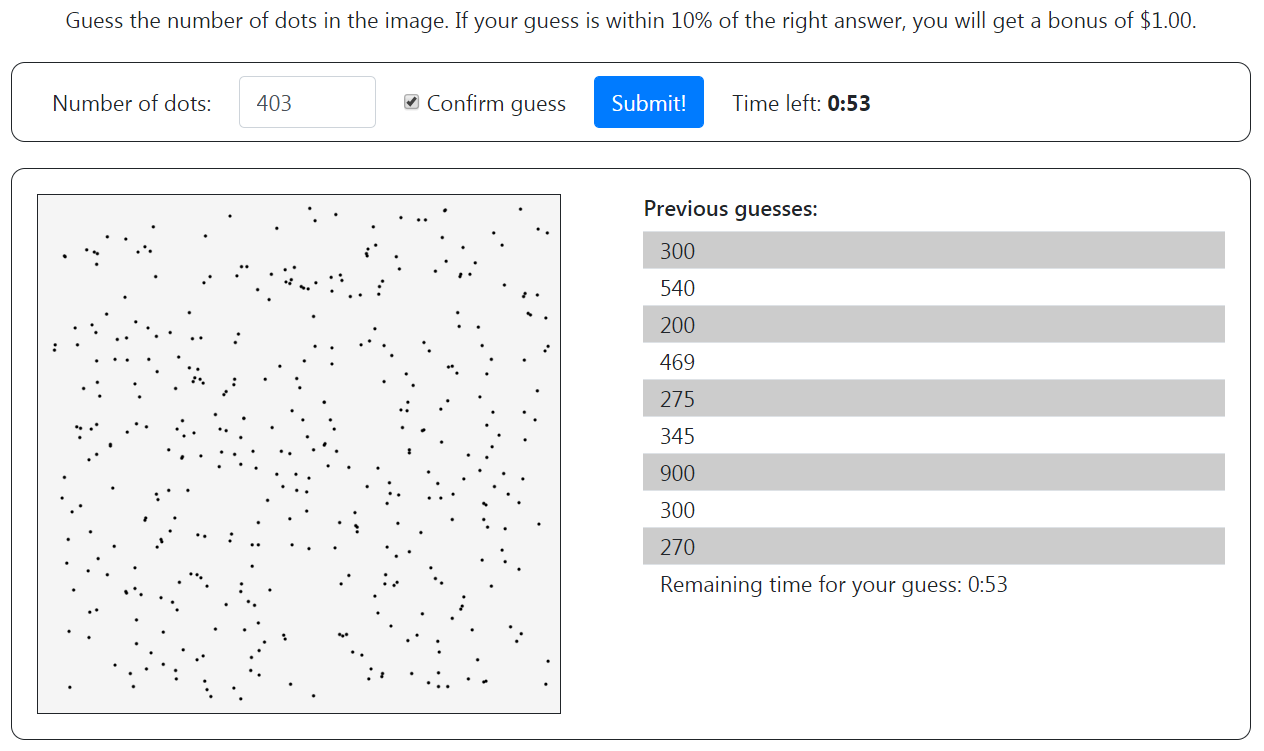
\includegraphics[width=.8\textwidth]{C:/Users/hjl161/Documents/Papers/WoT_github/images/FigS2.png}
\caption{Screendump of the choice-page in the dot-experiment with $d=403$ and $v=9$.}
\end{figure}

\begin{figure}
\centering
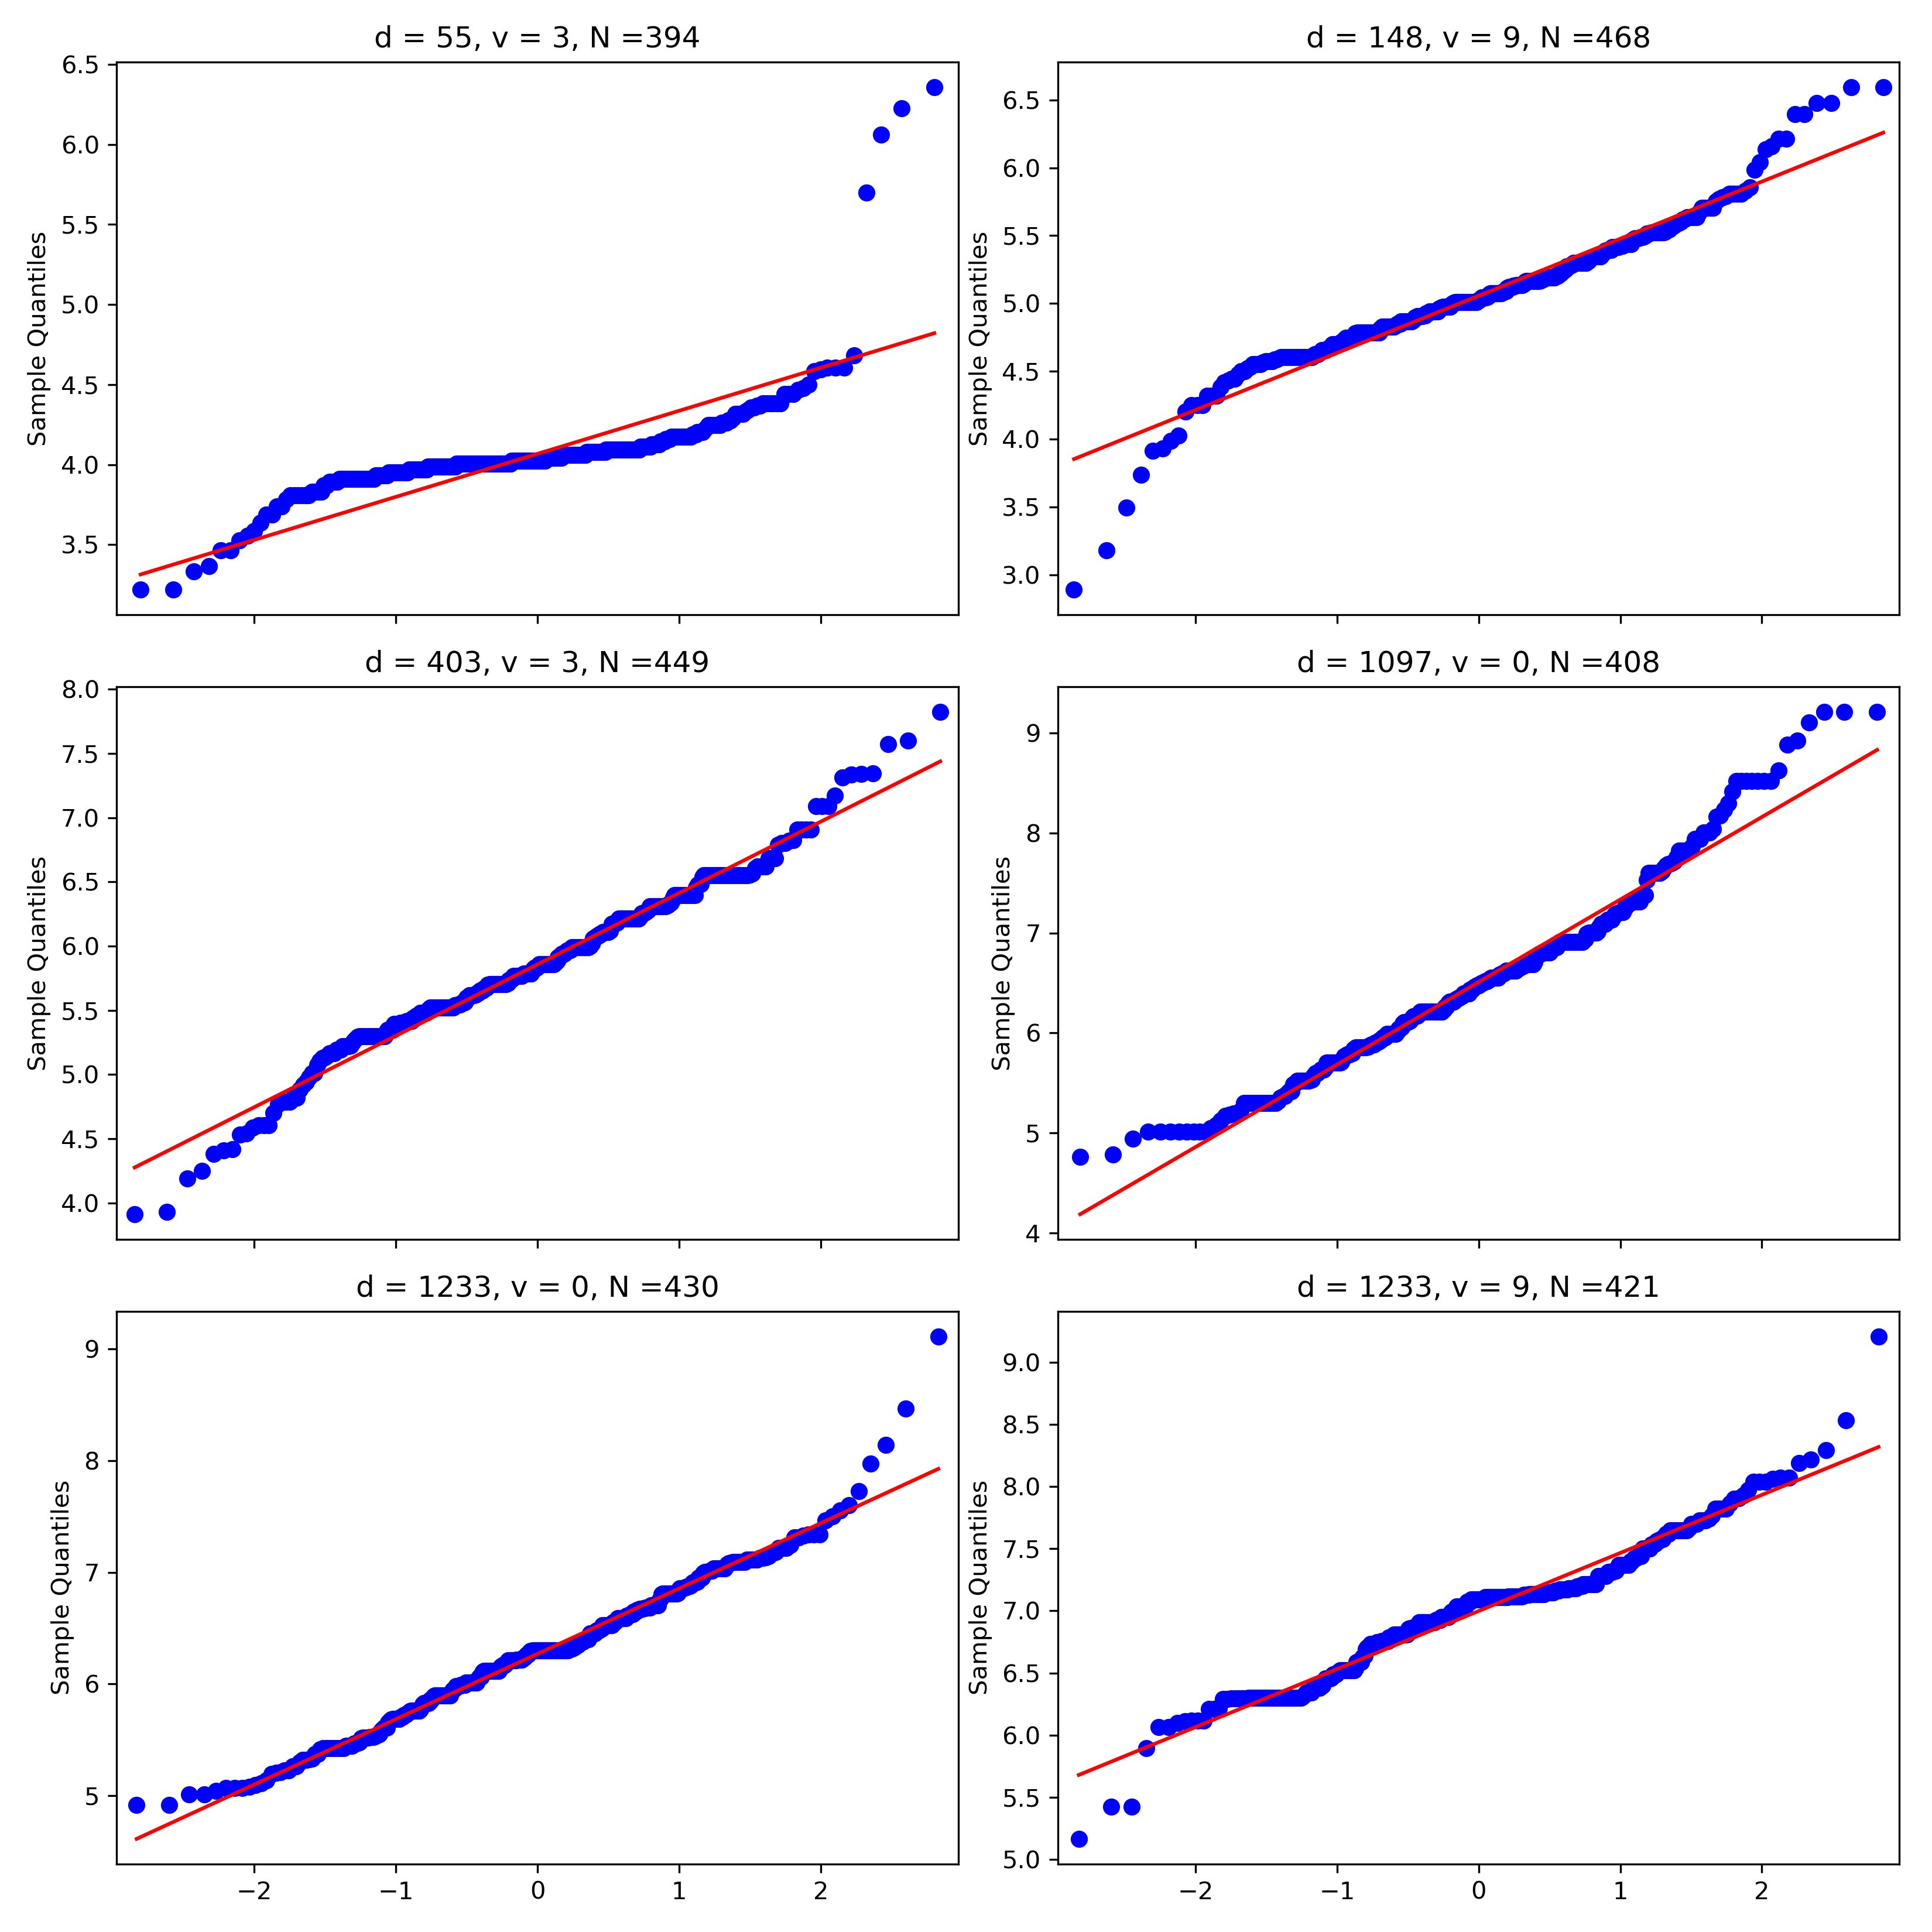
\includegraphics[width=.8\textwidth]{C:/Users/hjl161/Documents/Papers/WoT_github/plots/figS3.png}
\caption{QQ-plots of threads with log-transformed estimates indicating that distributions are only approximately log-normal.}
\end{figure}

\begin{figure}
\centering
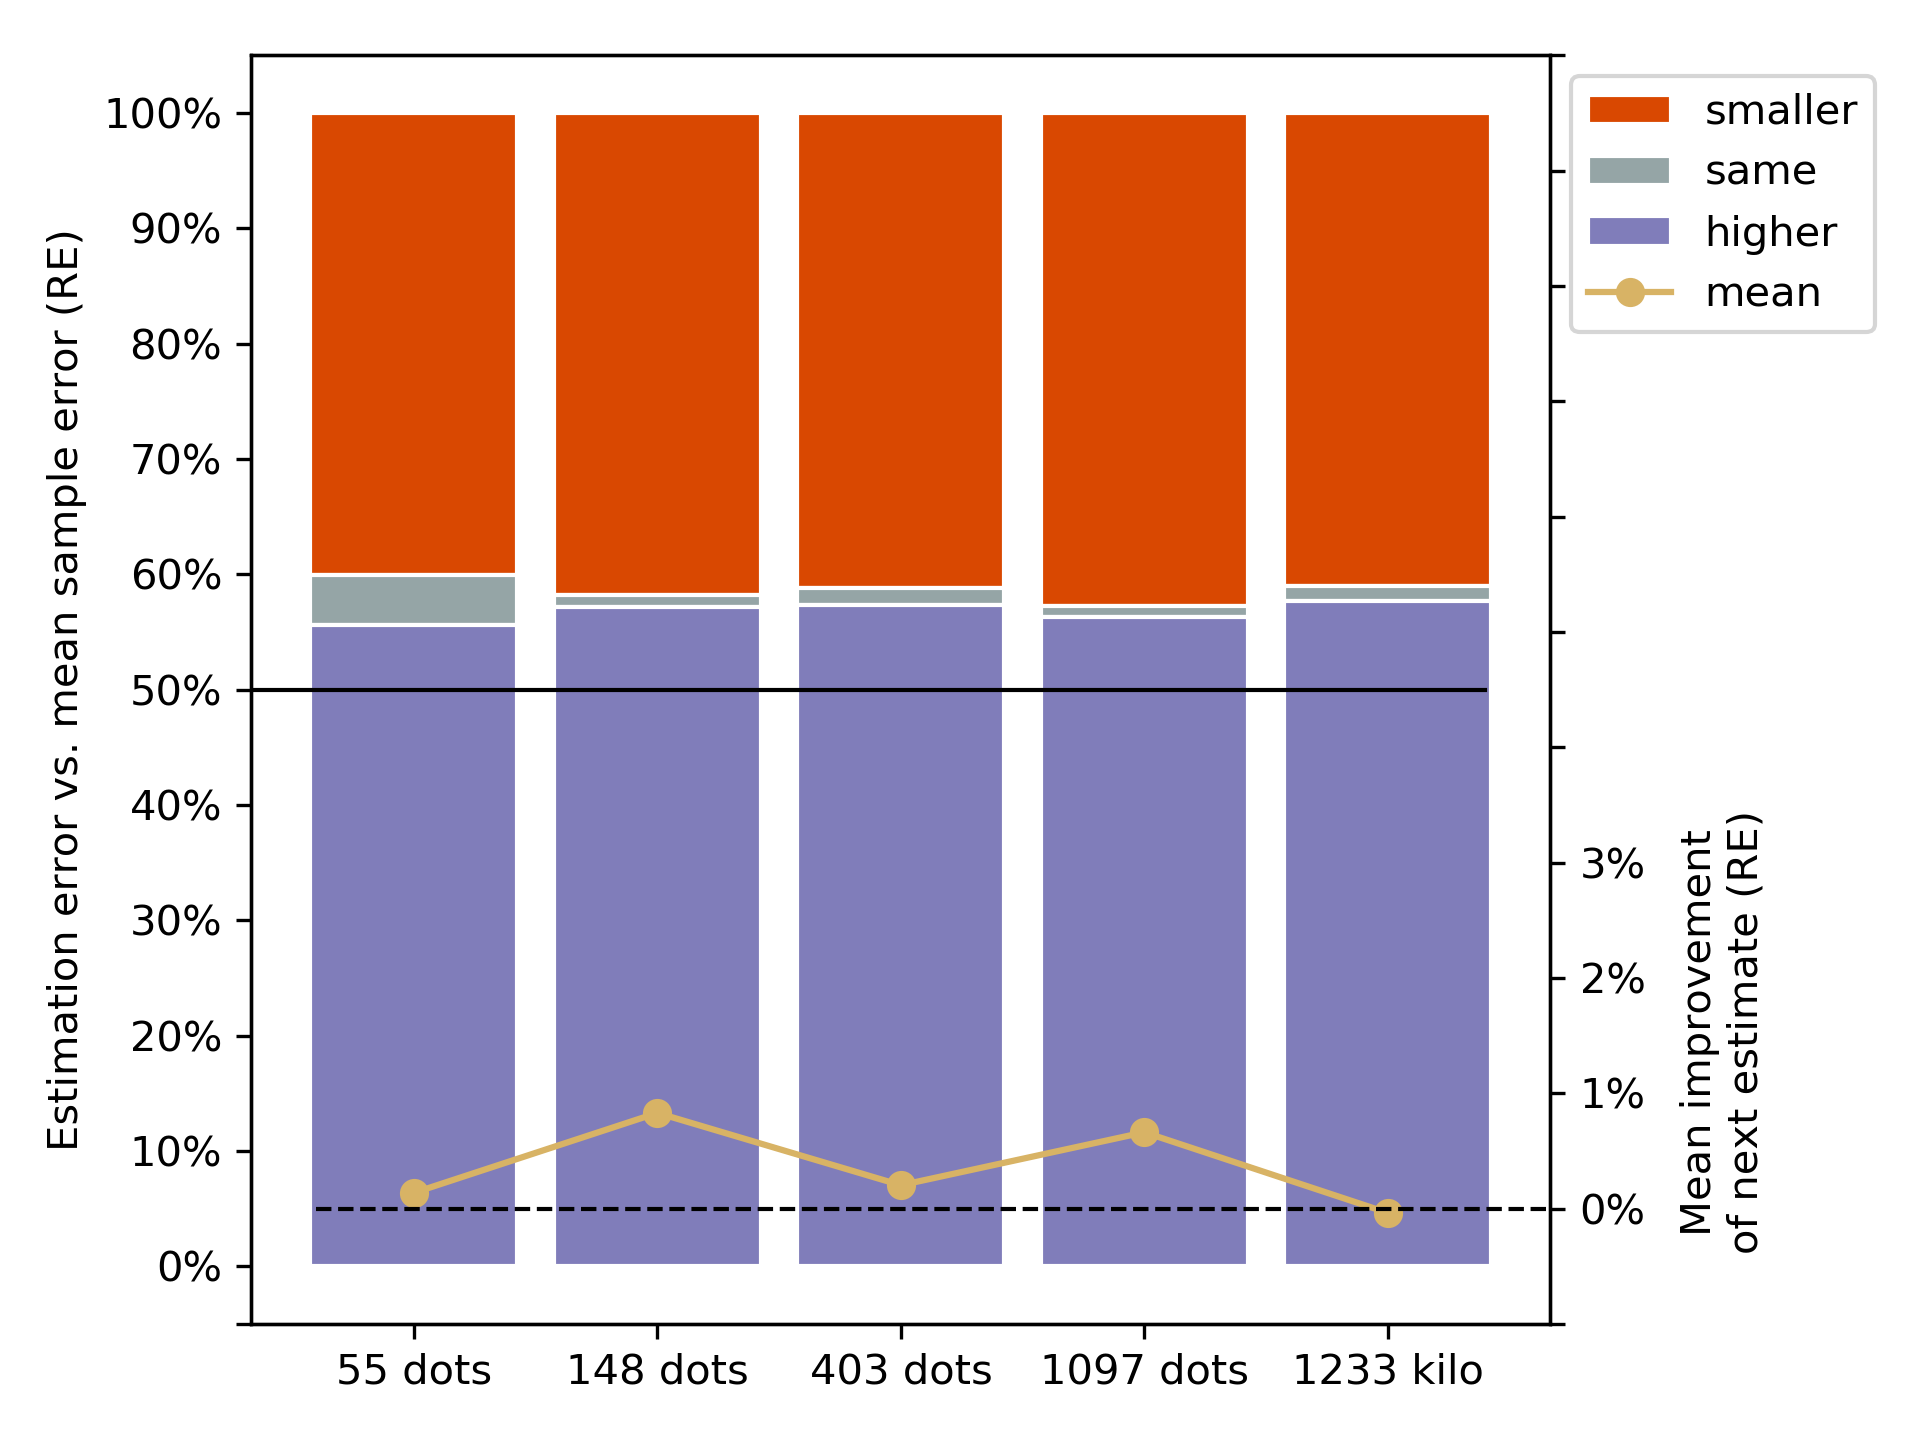
\includegraphics[width=.8\textwidth]{C:/Users/hjl161/Documents/Papers/WoT_github/plots/figS4.png}
\caption{Relative accuracy of estimates compared to their samples. Purple indicates the fraction of estimates with a smaller relative error than the mean relative error of the sample seen, where the relative error is defined as $|truth-estimates|/truth$. The grey bars indicate the fraction of estimates as good as their sample, and the red bars indicate the fraction of estimates with a higher error than the mean error rate of their sample. The last bar-plot shows the equivalent data from the ox-experiment. The line with markers shows the mean improvement over time measured as the difference in relative error.}
\end{figure}

\begin{figure}
\centering
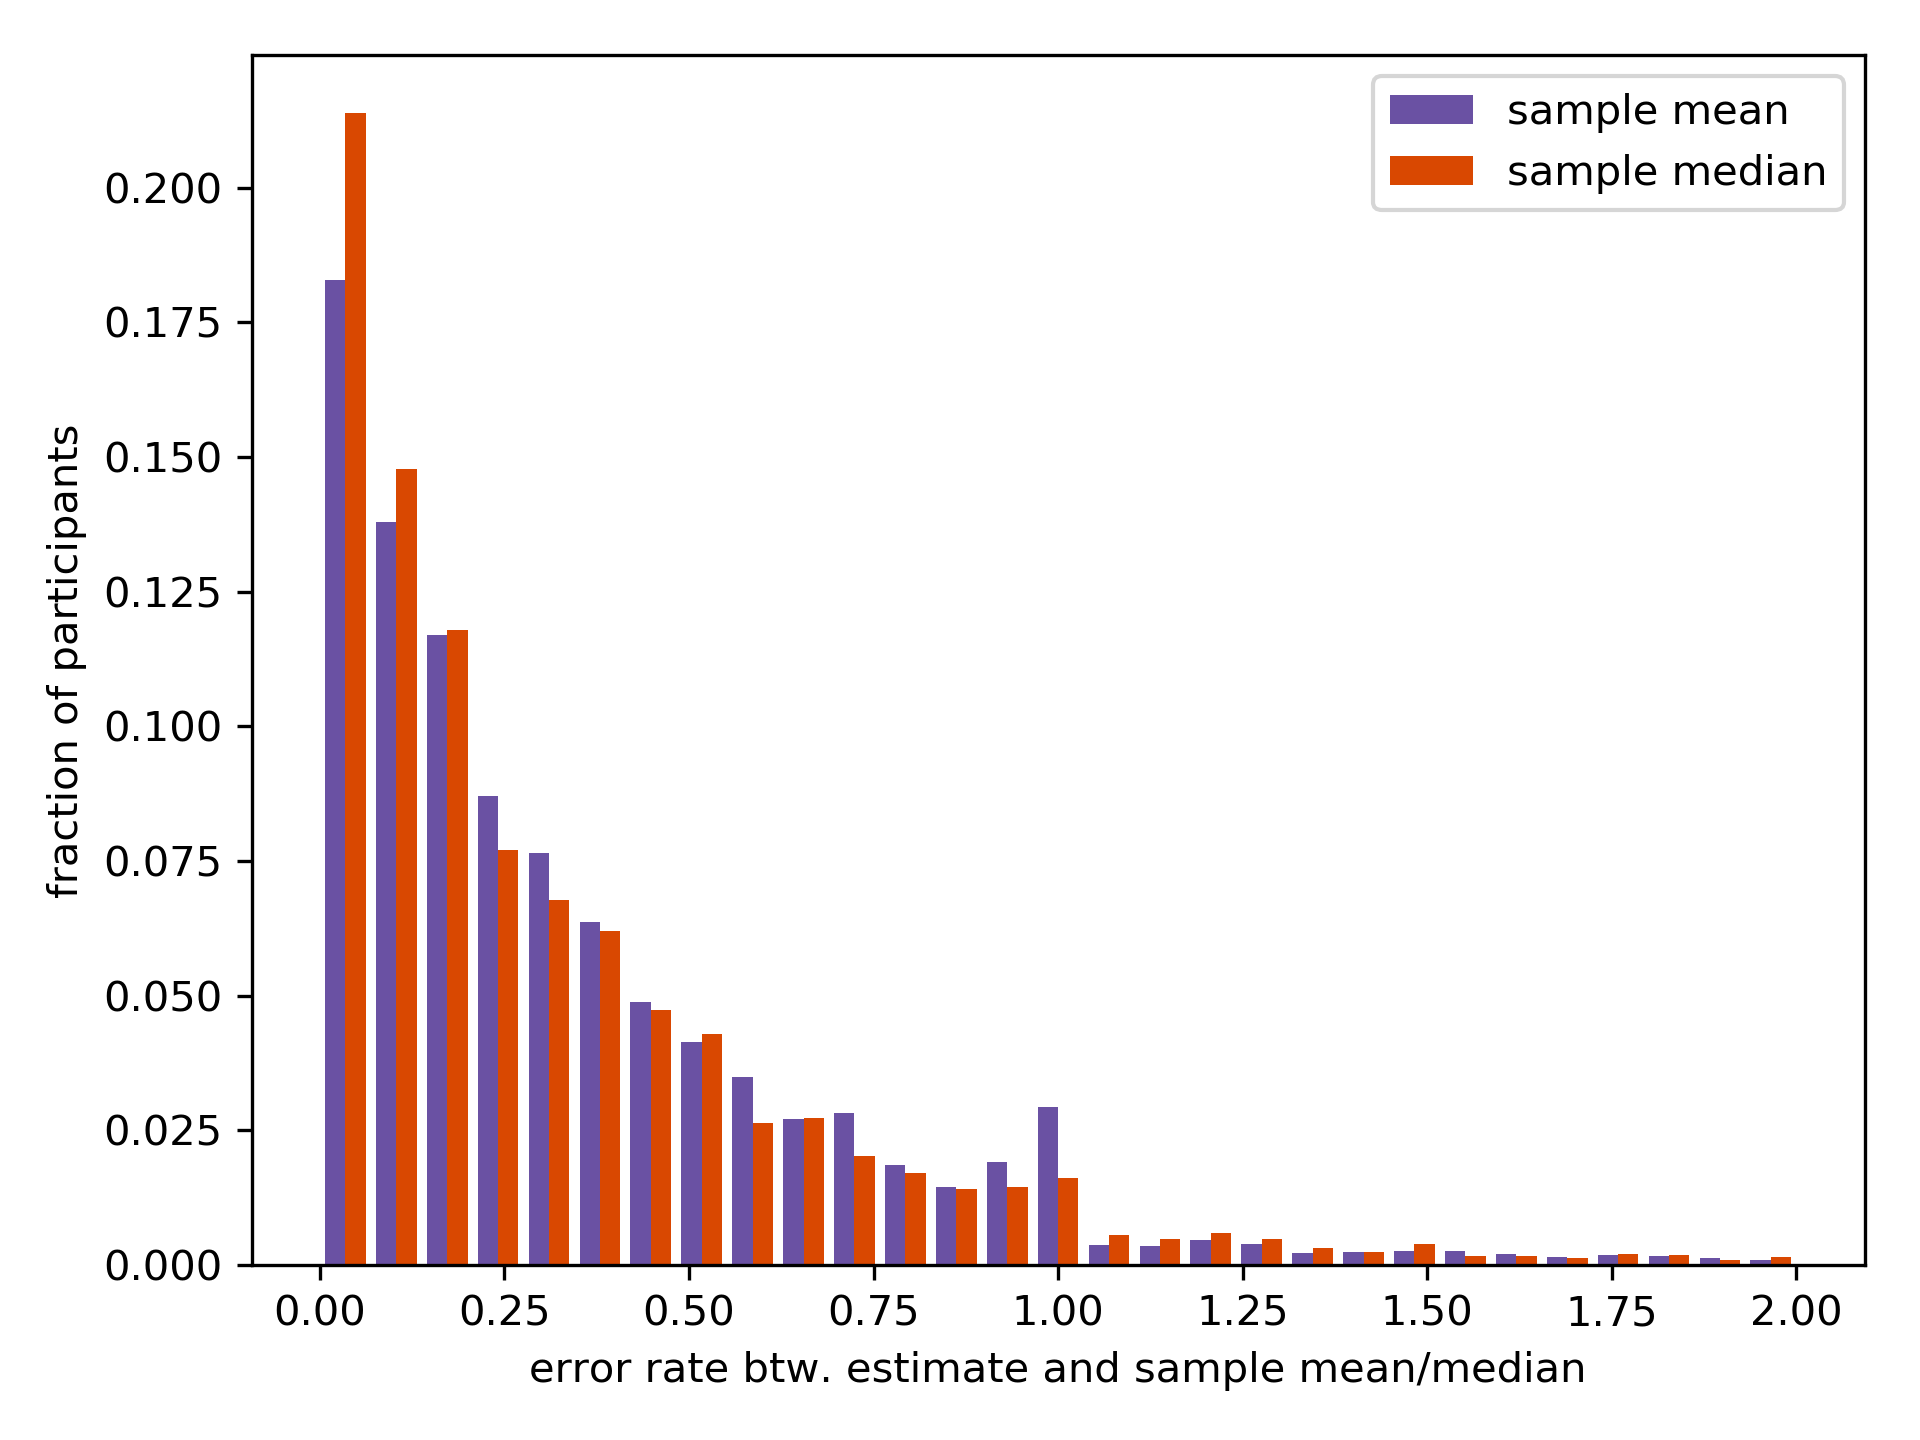
\includegraphics[width=.8\textwidth]{C:/Users/hjl161/Documents/Papers/WoT_github/plots/figS5.png}
\caption{Histogram of the error rates of individual estimates compared to the sample means/medians. It shows that many estimates are close to the average or the median of their sample (i.e. of the visible preceding estimates).}
\end{figure}

\begin{figure}
\centering
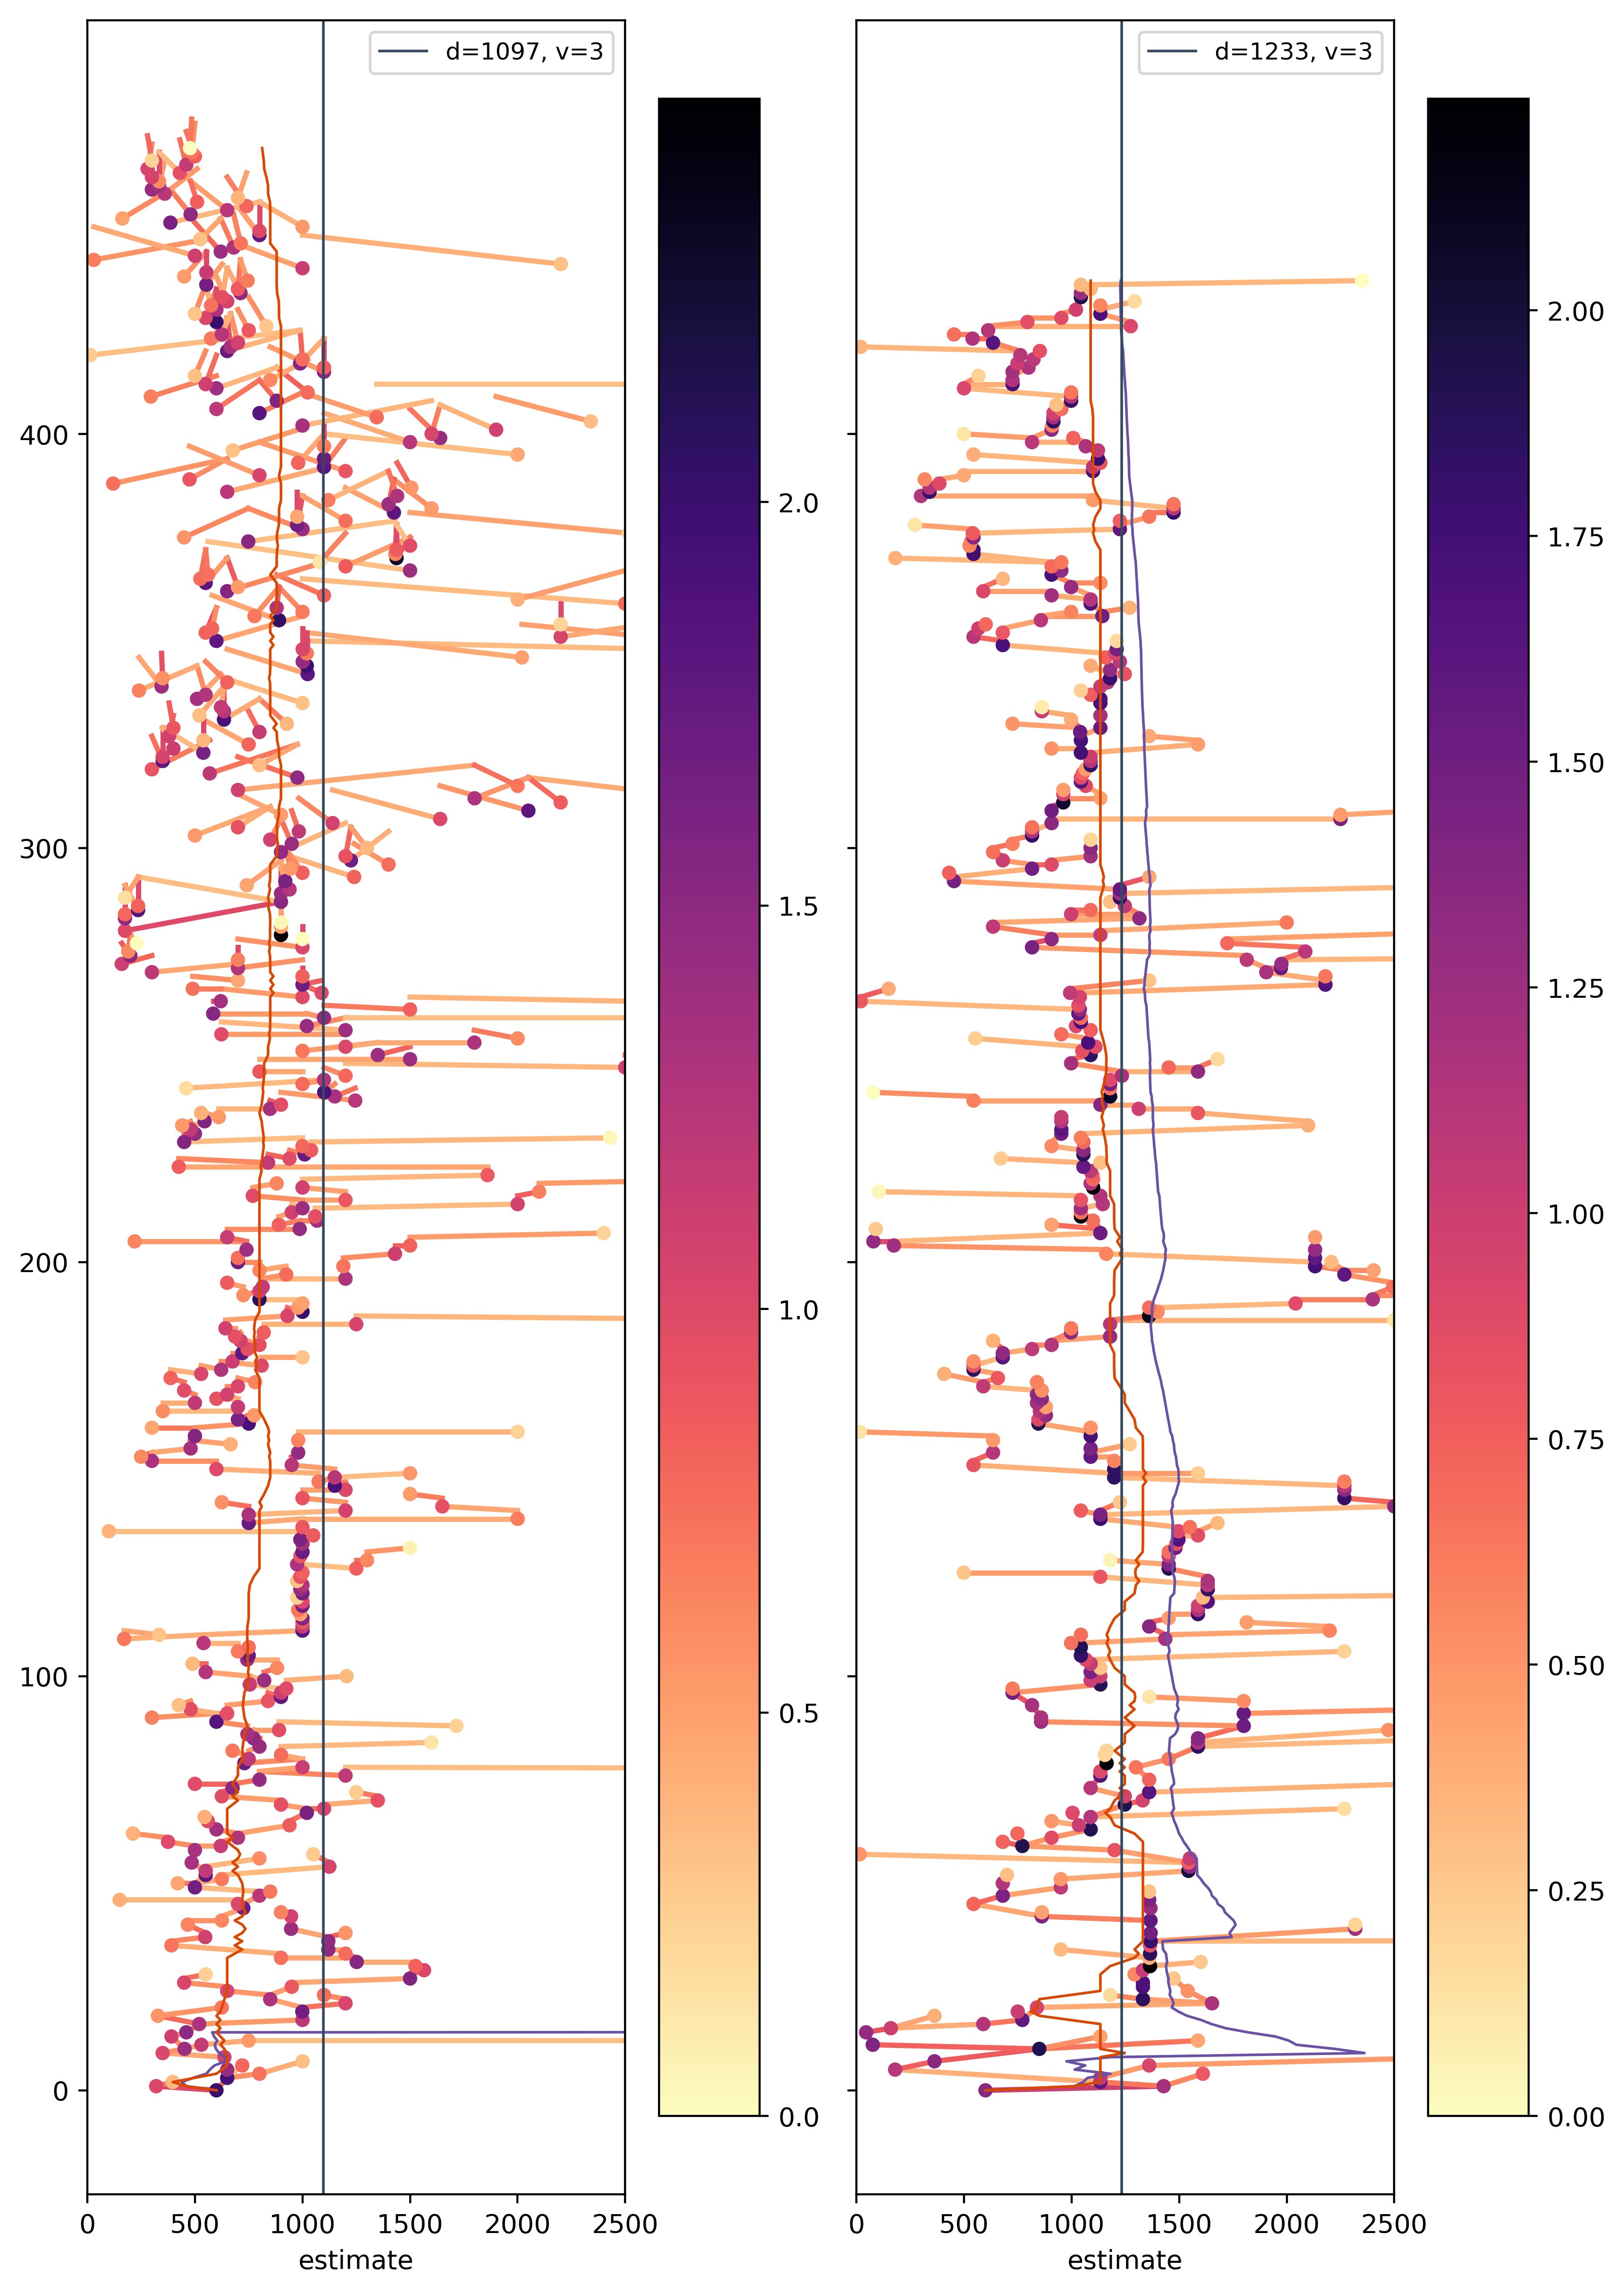
\includegraphics[width=.8\textwidth]{C:/Users/hjl161/Documents/Papers/WoT_github/plots/figS6.png}
\caption{The minimum spanning tree of two threads with $d=1097, v=3$ and $d=1233, v=3$, respectively, showing the development of individual estimates along the y-axis for dots and ox-threads. Line colors indicate the relative weight $w_{r,r-k}$ of the nearest preceding estimate, while dot colors specify the total social influence score, $s_r$, by participant $r$ upon succeeding estimates as calculated in the main text. The black line shows the true number of dots, the blue line shows the running average, and the red line shows the running median. The markedly more frequent instances of herding on the right can be seen as vertically aligned branches.}
\end{figure}

\begin{figure}
\centering
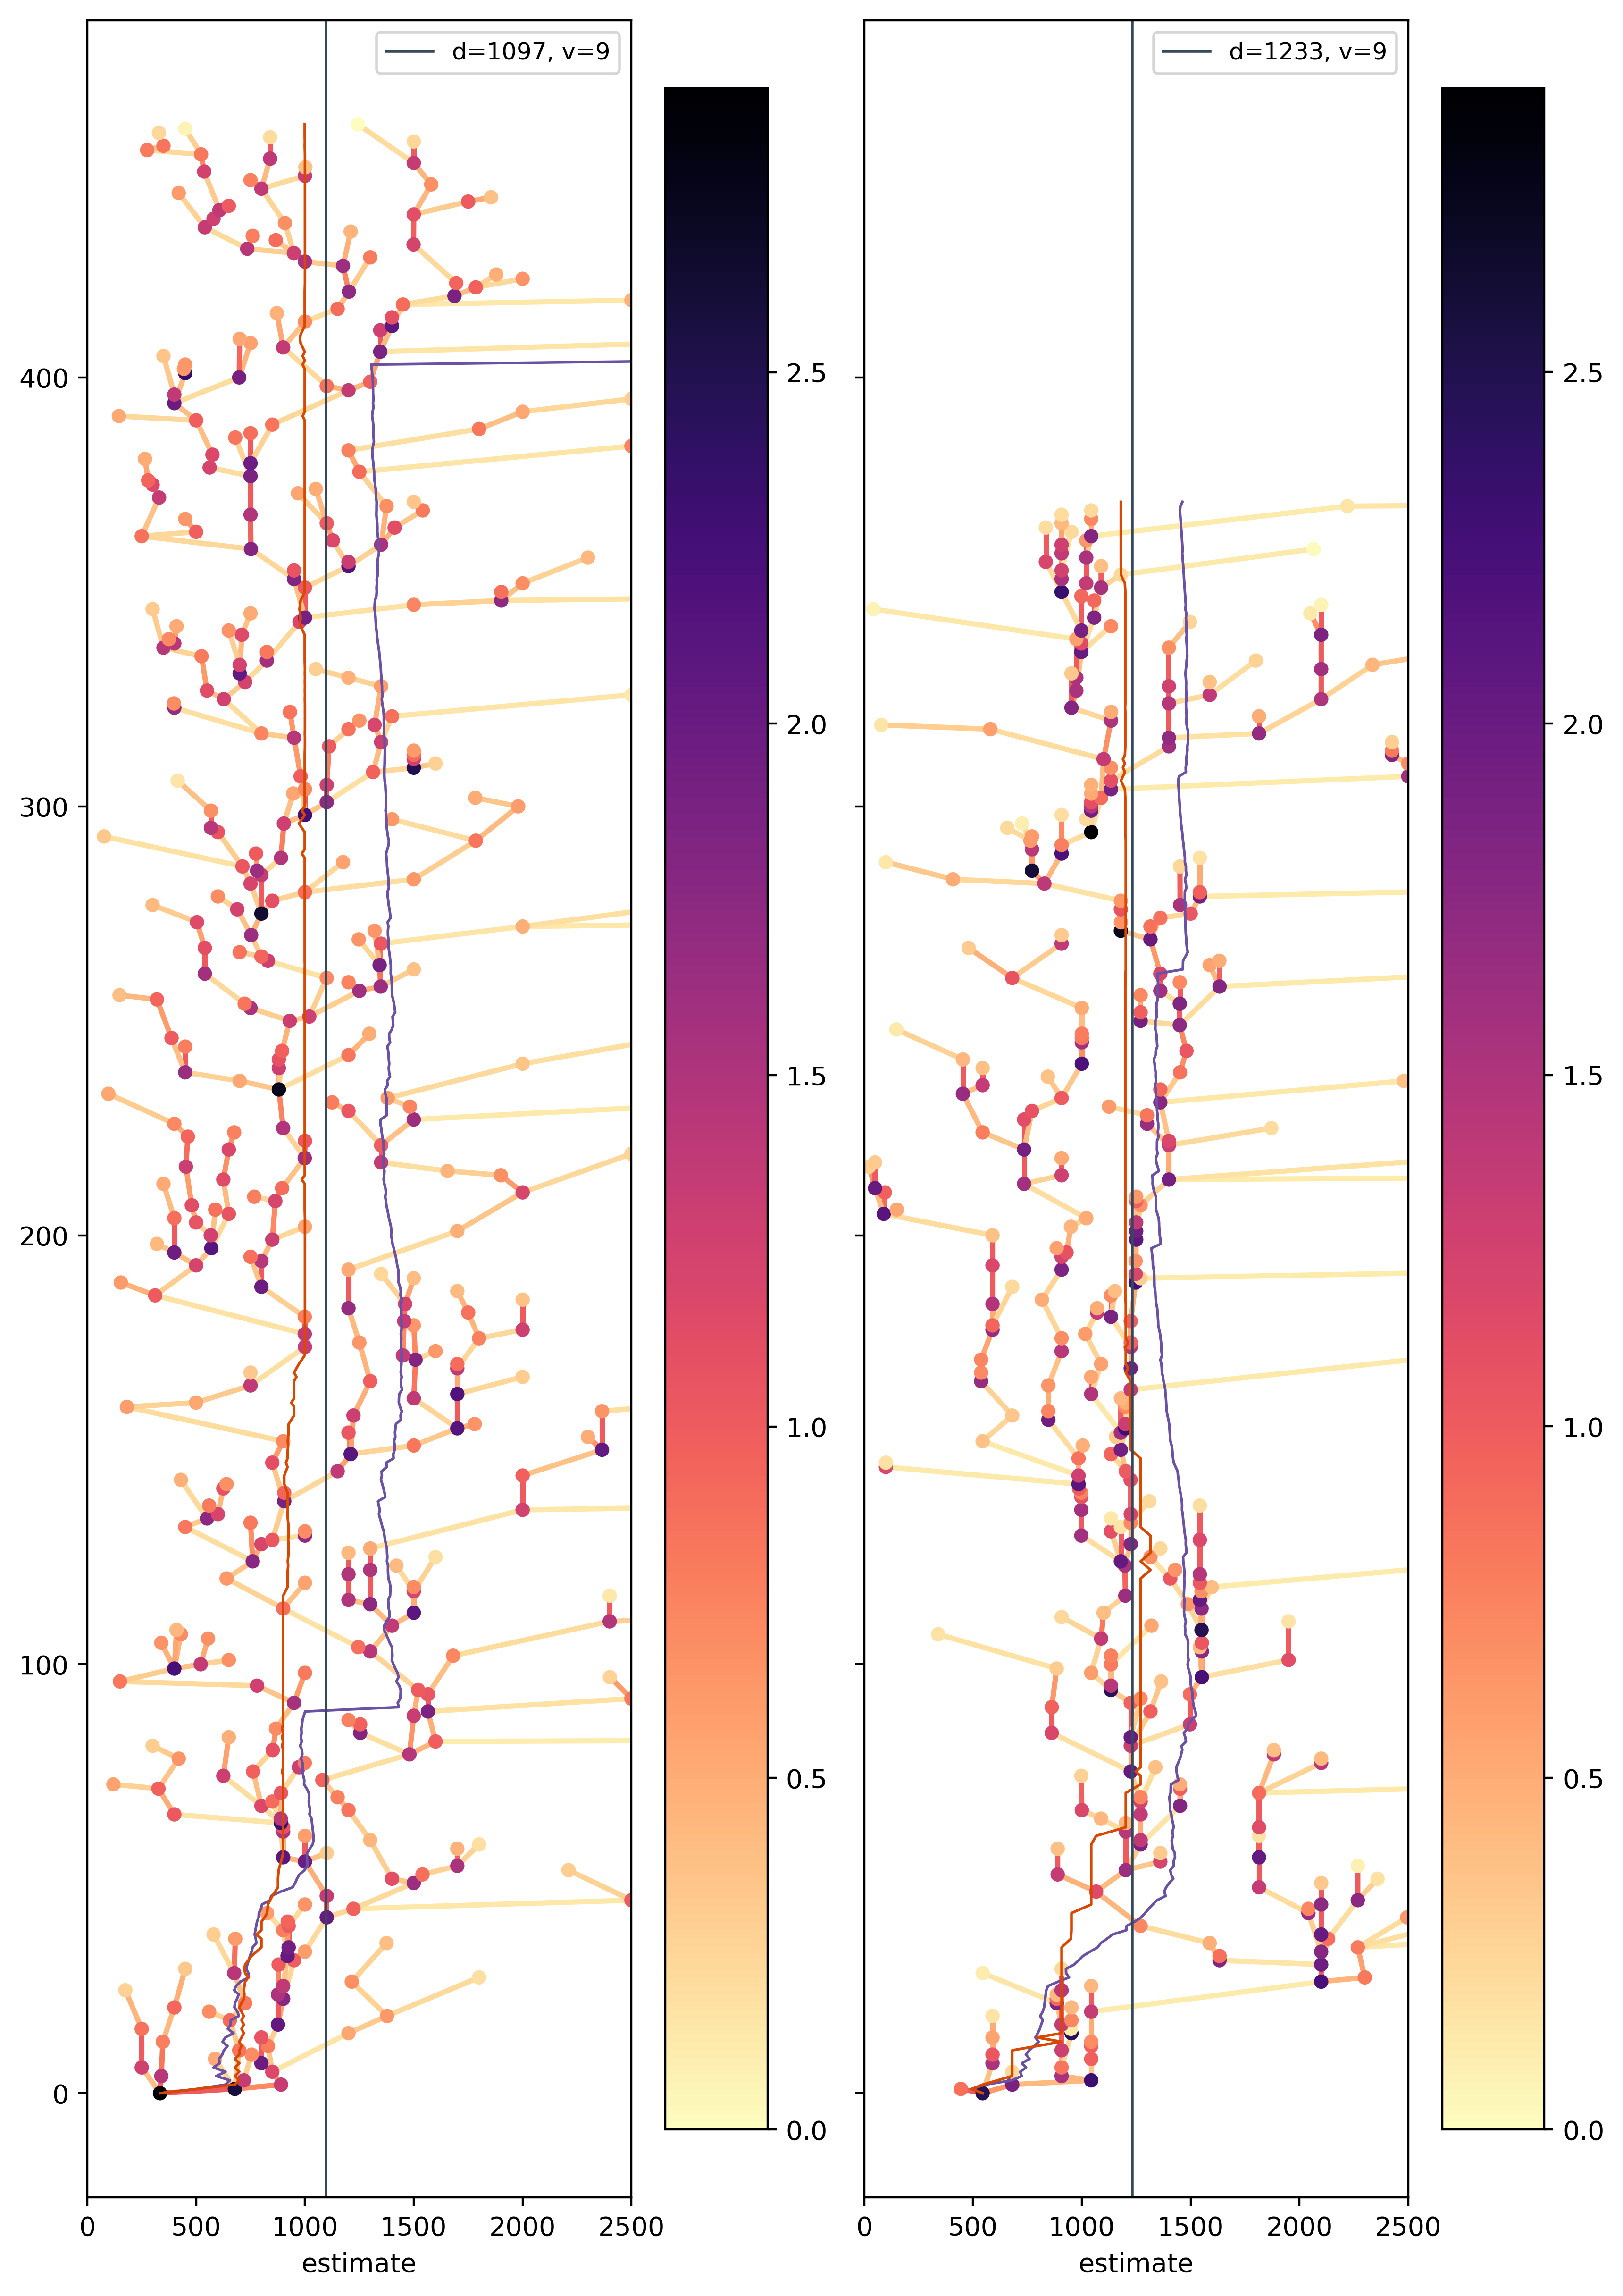
\includegraphics[width=.8\textwidth]{C:/Users/hjl161/Documents/Papers/WoT_github/plots/figS7.png}
\caption{The minimum spanning tree of two threads with $d=1097, v=9$ and $d=1233, v=9$, respectively, showing the development of individual estimates along the y-axis for dots and ox-threads. Line colors indicate the relative weight $w_{r,r-k}$ of the nearest preceding estimate, while dot colors specify the total social influence score, $s_r$, by participant $r$ upon succeeding estimates as calculated in the main text. The black line shows the true number of dots, the blue line shows the running average, and the red line shows the running median. Just like in figure S6, the bushy branches on the left and the sparse and fastigate branches on the right indicate that herding is much more pronounced when estimating the weight of an ox.}
\end{figure}

\begin{figure}
\centering
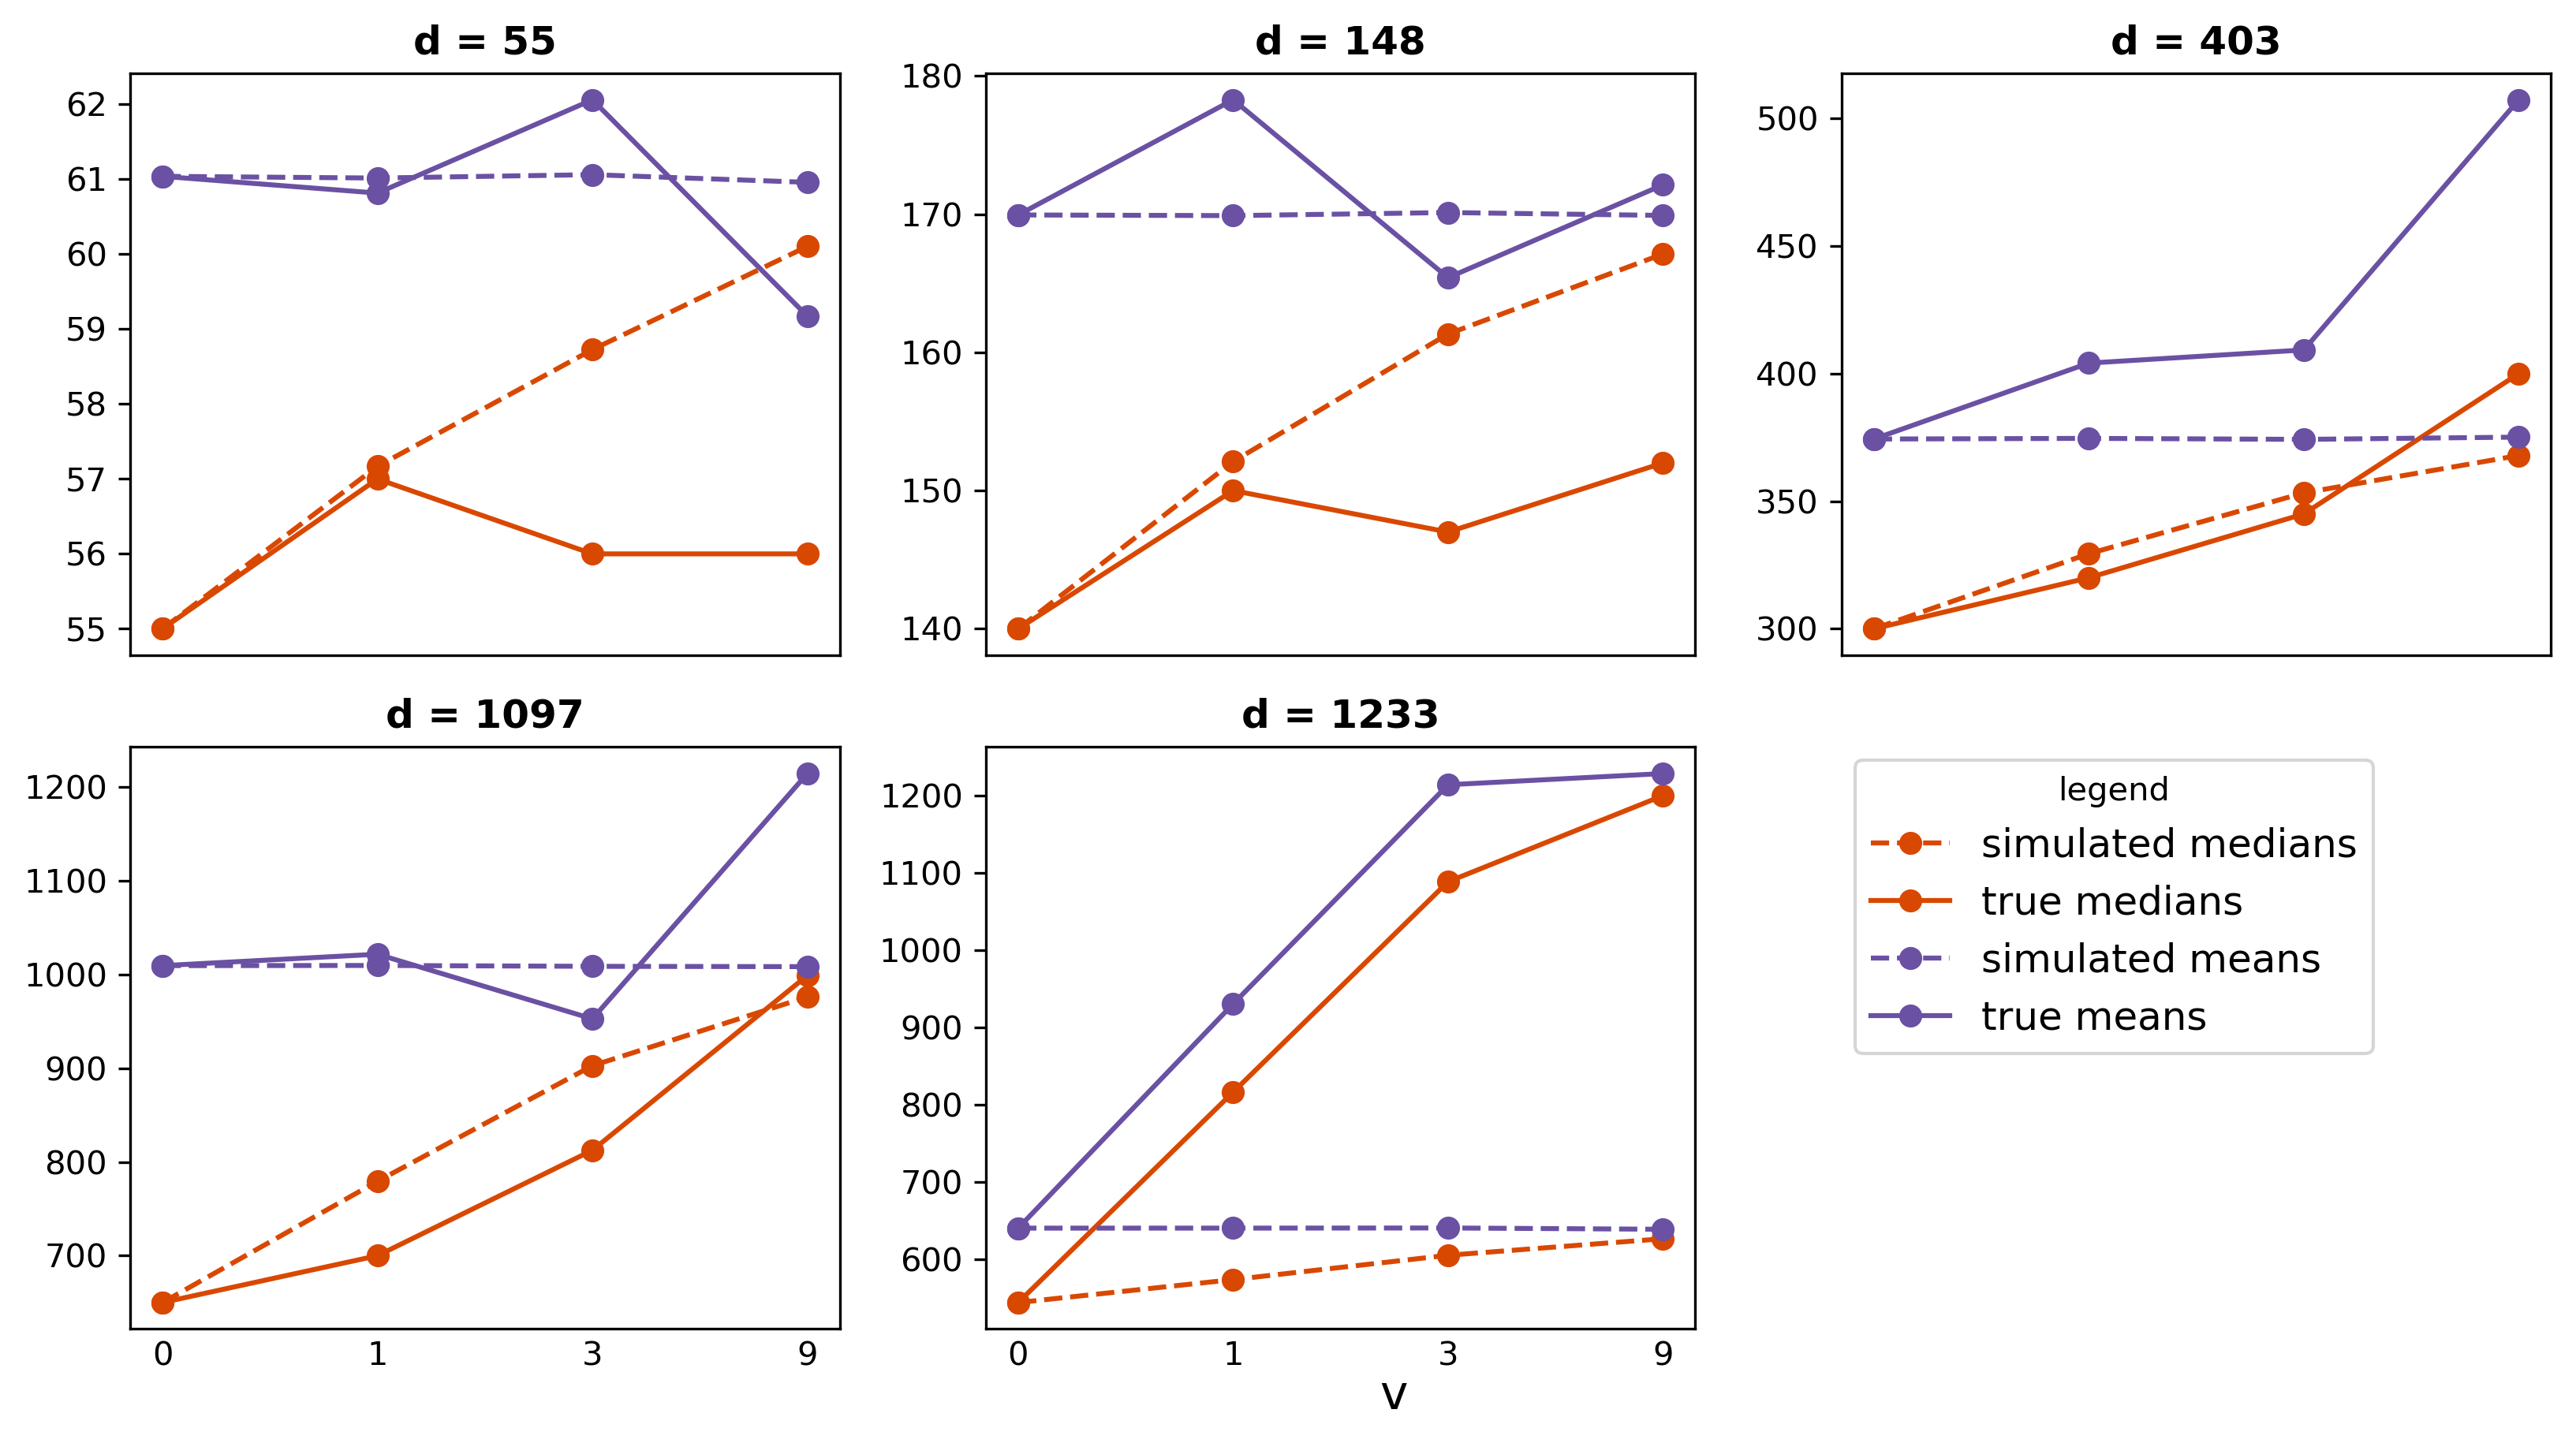
\includegraphics[width=.8\textwidth]{C:/Users/hjl161/Documents/Papers/WoT_github/plots/figS8.png}
\caption{Simulation results of a simple naïve learning model in which individuals report the average of all estimates seen including their own tentative ‘hunch’, drawn with replacement from the control treatments. Simulated results (dotted lines) are means over 1000 independent simulations. Actual medians from the experiments are show as solid lines.}
\end{figure}

\begin{figure}
\centering
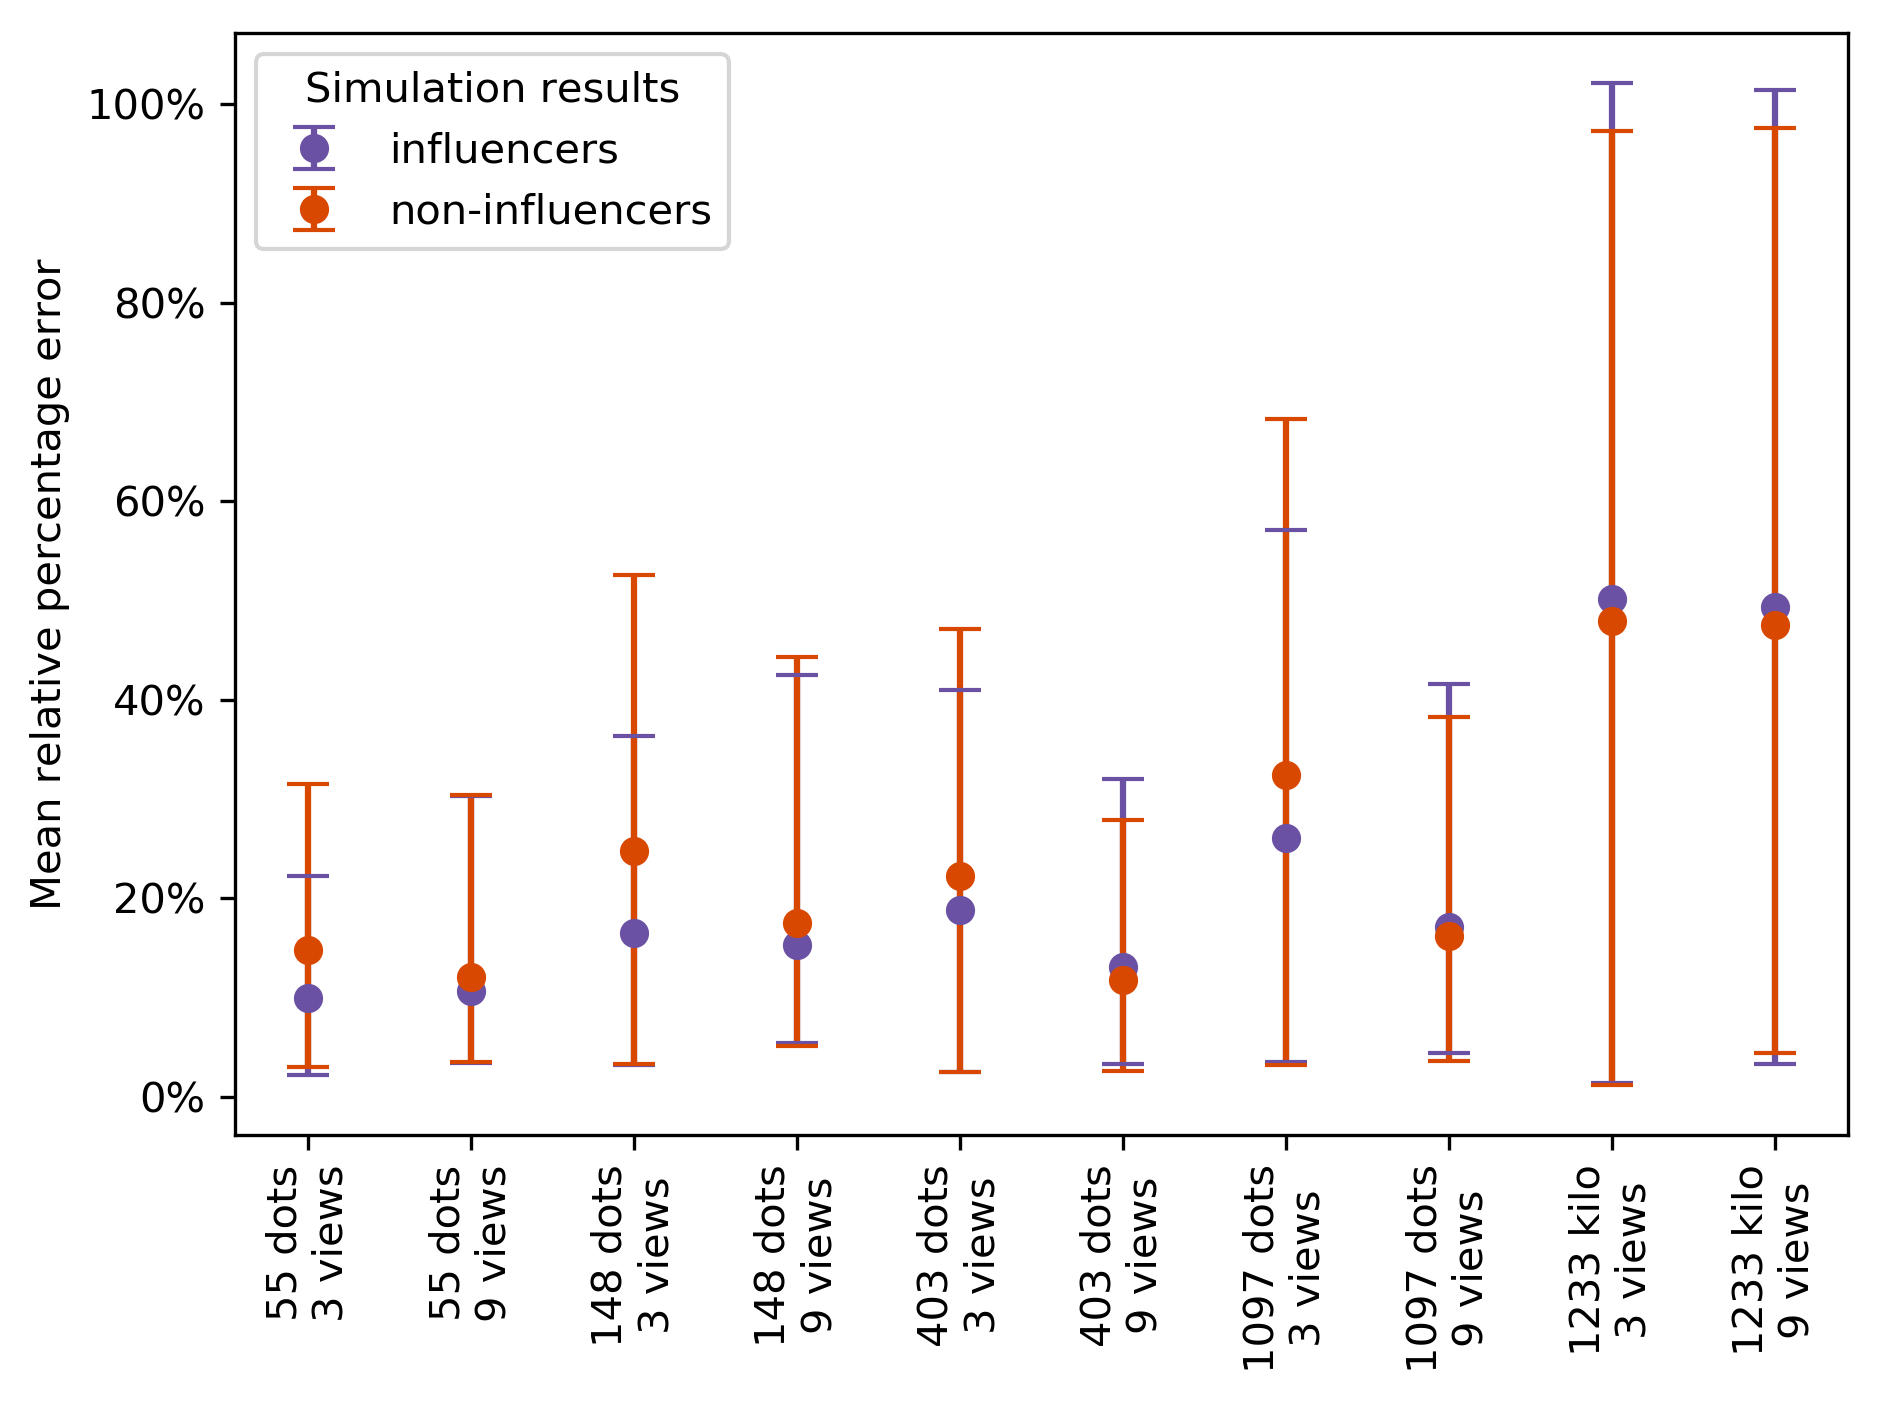
\includegraphics[width=.8\textwidth]{C:/Users/hjl161/Documents/Papers/WoT_github/plots/figS9.png}
\caption{Mean relative percentage errors of simulated data with 95\% confidence intervals for bootstrapped populations (N=1000) of mean relative errors of high- and low-influencers. The average difference in mean relative percentage errors across all 10 treatments as shown in the figure is 2\% - much less than the 23\% in figure 5 in the main text. Confidence intervals clearly indicate that participants’ ability to find and to follow accurate estimates is not due to the aggregation of their sample.}
\end{figure}

\begin{figure}
\centering
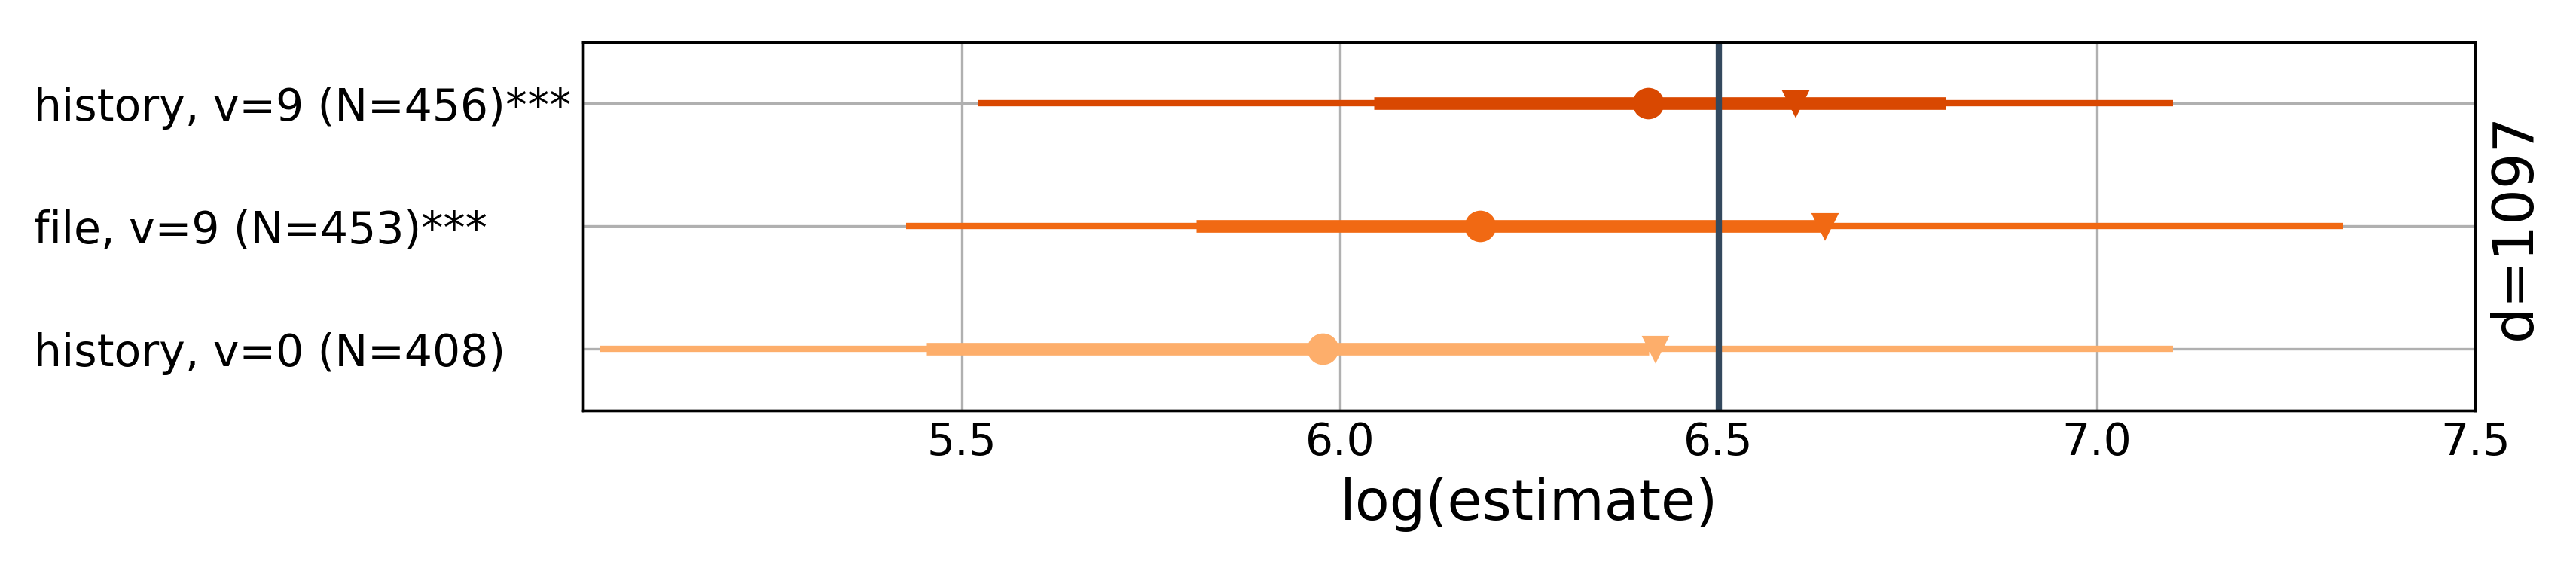
\includegraphics[width=.8\textwidth]{C:/Users/hjl161/Documents/Papers/WoT_github/plots/figS10.png}
\caption{Comparing the control treatment ($v=0$, bottom) and the normal history treatment of a thread with $d=1097$ dots (top) with a thread in which the $v=9$ estimates seen are drawn randomly from the control (middle).}
\end{figure}

\begin{table}\centering
\caption{Data Table of all threads. Legend: $d \in \{55$ dots, $148$ dots, $403$ dots , $1097$ dots, $1233$ kilo$\}$; $v$ = view count; method: \'history\'-threads show the preceding estimates as they have been recorded in the thread, while the file-condition shows nine random estimates from the control-treatment ($v=0$, session hal5jdl0); N = thread length; out = number of outliers removed; median = median of thread; mean = mean of thread; err-mean = error of thread mean; err-median = error of thread median; SD = standard deviation; CV = coefficient of variation; MAE = mean absolute error of estimates; skew = skewness; kurt = kurtosis; bonus = percentage of estimates within 10 \% of the true value, $d$.}
\begin{tabular}{rrllrrrrrrrrrrrr}
\hline
    d &   v & method   & thread   &   N &   out &   median &    mean &   err-med &   err-mean &      SD &   CV &   MAE &   skew &   kurt &   bonus \\
\hline
   55 &   0 & history  & fscmakcz & 464 &     8 &    55    &   61.04 &      0    &       0.11 &   33.78 & 0.55 &  0.21 &   9.54 & 118.7  &       61.18 \\
   55 &   1 & history  & hs6bovtz & 477 &     5 &    57    &   60.82 &      0.04 &       0.11 &   28.88 & 0.47 &  0.2  &  12.01 & 198.3  &       55.93 \\
   55 &   3 & history  & 3cda8qpn & 405 &    11 &    56    &   62.06 &      0.02 &       0.13 &   42.13 & 0.68 &  0.19 &   9.71 & 101.86 &       64.21 \\
   55 &   9 & history  & bvpj37io & 476 &     2 &    56    &   59.17 &      0.02 &       0.08 &   18.56 & 0.31 &  0.16 &   6.39 &  68.09 &       55.06 \\
  148 &   0 & history  & dwnjf9mb & 464 &    10 &   140    &  169.94 &      0.05 &       0.15 &  133.44 & 0.79 &  0.47 &   4.53 &  30.84 &       21.81 \\
  148 &   1 & history  & ehaxc7lu & 435 &     6 &   150    &  178.28 &      0.01 &       0.2  &  154.14 & 0.86 &  0.44 &   5.41 &  35.63 &       25.17 \\
  148 &   3 & history  & ck291lk5 & 466 &     9 &   147    &  165.4  &      0.01 &       0.12 &  112.79 & 0.68 &  0.36 &   6.02 &  50.01 &       22.98 \\
  148 &   9 & history  & 2hxe3g0w & 473 &     5 &   152    &  172.12 &      0.03 &       0.16 &   86.09 & 0.5  &  0.36 &   2.99 &  13.65 &       24.36 \\
  403 &   0 & history  & hqx0v7t5 & 473 &    12 &   300    &  374.36 &      0.26 &       0.07 &  333.27 & 0.89 &  0.52 &   4.54 &  32.7  &        8.03 \\
  403 &   1 & history  & 9bbkjlye & 469 &    10 &   320    &  404.13 &      0.21 &       0    &  350.03 & 0.87 &  0.49 &   5    &  34.91 &        8.06 \\
  403 &   3 & history  & 5du4txa7 & 455 &     6 &   345    &  409.28 &      0.14 &       0.02 &  266.89 & 0.65 &  0.44 &   3.01 &  14.9  &       11.36 \\
  403 &   9 & history  & spw8qdcd & 470 &     7 &   400    &  507.33 &      0.01 &       0.26 &  480.55 & 0.95 &  0.6  &   3.97 &  19.69 &       10.37 \\
 1097 &   0 & history  & hal5jdl0 & 423 &    15 &   650    & 1009.53 &      0.41 &       0.08 & 1320.5  & 1.31 &  0.7  &   4.15 &  20.91 &       10.05 \\
 1097 &   1 & history  & huyygtho & 461 &    11 &   750    & 1036.43 &      0.32 &       0.06 & 1073.33 & 1.04 &  0.59 &   4.22 &  25.09 &        9.33 \\
 1097 &   1 & history  & z0rvh02v & 473 &    17 &   641    & 1007.18 &      0.42 &       0.08 & 1332.51 & 1.32 &  0.66 &   4.93 &  28.73 &        8.99 \\
 1097 &   3 & history  & hhb0if6e & 470 &     6 &   812.5  &  952.73 &      0.26 &       0.13 &  746.16 & 0.78 &  0.43 &   5.71 &  54.61 &       20.69 \\
 1097 &   9 & file     & 699h8rze & 460 &     7 &   800    & 1263.08 &      0.27 &       0.15 & 1455.33 & 1.15 &  0.71 &   3.61 &  15.52 &       10.15 \\
 1097 &   9 & history  & wv4xujg7 & 460 &     4 &   999    & 1214.52 &      0.09 &       0.11 &  937.21 & 0.77 &  0.53 &   2.95 &  12.46 &       13.6  \\
 1233 &   0 & history  & gaijydul & 181 &     5 &   533.2  &  595.32 &      0.57 &       0.52 &  389.64 & 0.65 &  0.56 &   2.99 &  16.21 &        5.11 \\
 1233 &   0 & history  & ha6r7s1x & 271 &    17 &   544.31 &  671.9  &      0.56 &       0.46 &  696.36 & 1.04 &  0.56 &   7.93 &  85.7  &        7.87 \\
 1233 &   1 & history  & jizlqbb0 & 411 &    19 &   793.79 &  932.3  &      0.36 &       0.24 &  680.46 & 0.73 &  0.46 &   5.12 &  50.58 &        8.93 \\
 1233 &   1 & history  & kygak6r7 & 154 &     2 &   907.18 &  926.15 &      0.26 &       0.25 &  445.43 & 0.48 &  0.35 &   0.77 &   1.08 &       23.68 \\
 1233 &   3 & history  & 44qx5qq5 & 438 &    11 &  1088.62 & 1227.35 &      0.12 &       0    &  801.84 & 0.65 &  0.35 &   7.9  & 107.55 &       18.74 \\
 1233 &   3 & history  & nuf4ogmf & 332 &    17 &  1081.8  & 1195.98 &      0.12 &       0.03 &  856.41 & 0.72 &  0.4  &   5.83 &  55.74 &       19.68 \\
 1233 &   9 & history  & i0x2cimn & 210 &    15 &  1179.34 & 1118.21 &      0.04 &       0.09 &  442.36 & 0.4  &  0.26 &   1.29 &   3.34 &       40    \\
 1233 &   9 & history  & no1x9itu & 396 &    13 &  1179.34 & 1402.17 &      0.04 &       0.14 & 1007.03 & 0.72 &  0.41 &   5.2  &  40.25 &       21.41 \\
 1233 &   9 & history  & uhu19909 & 141 &     4 &  1202.02 & 1193.37 &      0.03 &       0.03 &  955.42 & 0.8  &  0.35 &   6.31 &  51.77 &       36.5  \\
\hline
 &&&& 10.808 & 254 &&&&&&&&& \\
\bottomrule
\end{tabular}
\end{table}\label{table:S1}

%%% Add this line AFTER all your figures and tables
\FloatBarrier

\dataset{dots.csv}{Anonymized data set of all dots-experiments. Parameters: task = type of experiment; d = number of dots in image; v = number of visible preceding estimates; session = thread name; code = unique identifier of participant; id = participant id in thread; order = order in which participants enter the queue; hist = list of preceding id's having made an estimate; guess = estimate by participant; bonus = payoff in dollars if estimate was within 10\% of d.}

\dataset{ox.csv}{Anonymized data set of all ox-experiments. Parameters: task = type of experiment; d = weight of the ox (in kilo); v = number of visible preceding estimates; session = thread name; code = unique identifier of participant; id = participant id in thread; order = order in which participants enter the queue; hist = list of preceding id's having made an estimate; guess = estimate by participant; pound = 1 if estimate was made in lb, 0 if estimate was made in kg; bonus = payoff in dollars if estimate was within 10\% of d.}

\bibliography{biblio_wot}

\end{document}